\documentclass[11pt]{article}

\usepackage[margin=1.05in]{geometry}
\usepackage{amsmath,amssymb,mathtools}
\usepackage{booktabs}
\usepackage{microtype}
\usepackage{hyperref}
\usepackage{xcolor}
\usepackage{tikz}
\usetikzlibrary{arrows.meta,positioning,calc}

\hypersetup{
  colorlinks=true,
  linkcolor=blue!70!black,
  citecolor=blue!70!black,
  urlcolor=blue!70!black
}

% --- Notation (match repo conventions) ---
\newcommand{\phig}{\varphi}
\newcommand{\lnphi}{\ln\phig}
\newcommand{\logphi}{\log_{\phig}}
\newcommand{\muStar}{\mu_\star}
\newcommand{\Ecoh}{E_{\mathrm{coh}}}
\newcommand{\Fgap}{\mathrm{gap}}
\newcommand{\fRG}{f^{\mathrm{RG}}}
\newcommand{\fRec}{f^{\mathrm{Rec}}}
\newcommand{\Zidx}{Z}
\newcommand{\tildeQ}{\tilde Q}
\newcommand{\mRS}{m_{RS}}
\newcommand{\mskel}{m_{\mathrm{skel}}}
\newcommand{\mdata}{m_{\mathrm{data}}}
\newcommand{\mPred}{m_{\mathrm{pred}}}
\newcommand{\muT}{\mu_{\mathrm{target}}}
\newcommand{\RGPolicy}{\texttt{RS\_CANONICAL\_2025\_Q4}}

\title{\textbf{Standard-Model Masses from Octave Closure and Integer Baselines}\\[0.3em]
\large Single-anchor formulation with explicit transport hygiene}
\author{(draft; internal circulation)}
\date{\today}

\begin{document}
\maketitle

\begin{abstract}
\noindent
The Standard Model treats fermion masses as inputs (Yukawa couplings) rather than outputs.
Recognition Science (RS) proposes that stable particles correspond to stable recognition boundaries whose mass values
are organized by (i) a forced eight-tick closure (\emph{Octave}) and (ii) a scale-coordinate on a $\phig$-ladder.
At a single common anchor scale $\muStar$, the charged-fermion spectrum is described by a sector-global yardstick
and an explicit charge$\to$integer$\to$band map:
\[
  m_{RS}(i;\muStar) = A_{\mathrm{sector}(i)}\,\phig^{\,r_i - 8 + \Fgap(\Zidx_i)}.
\]
To compare to PDG scheme choices at other scales, Standard-Model renormalization-group (RG) running is used
\emph{only} as a transport factor; critically, we do not identify the RS band coordinate $\fRec(\Zidx)$ with the SM
transport exponent $\fRG(\mu_1,\mu_2)$.
All tables and checks in this draft are reproducible from the repository.
\end{abstract}

\tableofcontents
\newpage

\section{Introduction (motivation and paper spine)}
\subsection{What the Standard Model does and does not explain about masses}
In the Standard Model (SM), fermion masses arise from Yukawa couplings.
Those Yukawas are free inputs: the SM does not explain why the electron, muon, and tau have the numerical values they do,
nor why quarks cluster into three charge-families with large separations.
This motivates searching for \emph{structure}: a small set of organizing principles that place masses on a constrained spectrum.

\subsection{Recognition Science move: masses as ladder coordinates under forced closure}
Recognition Science (RS) starts from the premise that stable particles correspond to stable recognition boundaries.
A boundary is not only a ``thing'' but a repeatable recognition process; stability is therefore a question of discrete closure.
Two RS ingredients matter here:
\begin{itemize}
  \item \textbf{Octave (8-tick closure).} In a three-bit context space, full coverage requires $2^3=8$ states.
  Eight ticks is the minimal closure that can support stable periodicity.
  \item \textbf{$\phig$-ladder coordinate.} Physical scales are treated as coordinates in $\log_\phig$ units.
  We adopt $\phig$ as the log base because the RS mass law is expressed in $\phig$-powers; in this paper this is a
  declared coordinate convention (DEF). On such a ladder, integer shifts correspond to multiplying by $\phig$.
\end{itemize}
This paper’s spine is: \emph{at a single anchor scale}, charged fermion masses are described by sector-global integers plus an explicit
charge-index band coordinate.

\subsection{What this paper provides (deliverables)}
This draft is designed to be referee-resistant by making the claim contract explicit:
\begin{itemize}
  \item the anchor mass display law and its decomposition into (yardstick) $\times$ (rung skeleton) $\times$ (band coordinate),
  \item the derivation of sector yardstick integers from cube/wallpaper integers,
  \item the closed-form map $\Zidx\mapsto\Fgap(\Zidx)$ and its canonical values for charged families,
  \item a strict transport section whose entire purpose is to prevent the category error $\fRec=\fRG$,
  \item reproducible tables (auto-generated from the canonical repository spec).
\end{itemize}

\section{Scope, claims hygiene, and what is being tested}
\paragraph{Two tiers.}
We separate two kinds of work to prevent category errors.
\begin{itemize}
  \item \textbf{Tier A (anchor display).} A structural coordinate table at $\muStar$: it defines $A_{\mathrm{sector}}$, $\Fgap(\Zidx)$,
  and $m_{RS}(i;\muStar)$. This is \emph{not} a claim that $m_{RS}(\muStar)$ equals PDG pole masses.
  \item \textbf{Tier B (absolute leptons).} A separate pipeline (T9/T10) that predicts $(m_e,m_\mu,m_\tau)$ in MeV using additional
  structure (topological shift and derived steps). We include Tier B as a reproducible result table, but keep the transport hygiene
  rules identical.
\end{itemize}

\paragraph{Tag vocabulary.}
We use: \textbf{THEOREM (Lean)} for proved statements; \textbf{DEF (Lean)} for definitions; \textbf{CERT} for pinned external numerical
certificates; \textbf{VALIDATION} for comparisons to PDG/CODATA.

\paragraph{What this paper is \emph{not} claiming (up front).}
\begin{itemize}
  \item We do \emph{not} claim $\mRS(i;\muStar)$ equals PDG pole masses.
  \item We do \emph{not} claim the band coordinate is RG-invariant off-anchor.
  \item We do \emph{not} claim $\fRG=\fRec$; they are defined differently and have different typical magnitudes.
\end{itemize}

\paragraph{Parameter accounting (what can and cannot be called ``fit'').}
Tier A uses no per-species tuning knobs. The structural display depends on:
\begin{itemize}
  \item $\phig$ (scale unit),
  \item sector-global integers $B_{\mathrm{pow}}(\mathrm{sector})$ and $r_0(\mathrm{sector})$ (yardstick),
  \item a rung integer $r_i$ (species ladder coordinate),
  \item the integerized charge map $Q\mapsto \tildeQ=6Q \mapsto \Zidx$,
  \item the closed-form band coordinate $\Fgap(\Zidx)$,
  \item the octave reference shift $-8$ (coordinate origin),
  \item one global anchor scale $\muStar$ (a declared comparison convention).
\end{itemize}

\paragraph{Tier B constants (lepton absolute pipeline).}
The Tier B pipeline additionally uses:
\begin{itemize}
  \item a gap-weight constant $w_8 \approx 2.490569$ (DEF in Lean, with the normalized DFT-8 projection equality proved as a THEOREM: \texttt{IndisputableMonolith.Constants.GapWeight.ProjectionEquality.w8\_projection\_equality}),
  \item the fine-structure constant $\alpha$ derived from cube/wallpaper integers and $w_8$,
  \item topological shift and step formulas (derived from $\alpha$ and geometry).
\end{itemize}

Any comparison to PDG at a different $\muT$ necessarily introduces an \emph{explicit RG transport policy}
(scheme, thresholds, loop order), which must be declared and is not part of the RS structural law.

\paragraph{Non-circularity rule (operational).}
No measured $m_i$ may appear on the right-hand side of its own prediction. Any global calibration (if used) must be declared, frozen,
and validated on hold-outs.

\section{Definitions and notation (self-contained)}
\subsection{The \texorpdfstring{$\phig$}{phi}-ladder and log-scale coordinates}
Let $\phig=(1+\sqrt5)/2$ and $\logphi(x):=\ln(x)/\lnphi$.
We treat $\logphi(m)$ as a \emph{scale coordinate} on a $\phig$-ladder.

\subsection{Charge integerization and the band integer \texorpdfstring{$\Zidx$}{Z}}
Let $Q$ be electric charge in units of $e$ and define $\tildeQ := 6Q \in \mathbb Z$.
Define the charge-index integer map $\Zidx$ by
\begin{equation}
  \Zidx(Q,\mathrm{sector}) :=
  \begin{cases}
    \tildeQ^2 + \tildeQ^4, & \mathrm{sector}=\mathrm{lepton},\\
    4 + \tildeQ^2 + \tildeQ^4, & \mathrm{sector}=\mathrm{quark}.
  \end{cases}
  \label{eq:Zmap}
\end{equation}
This gives the three charged-family values:
\[
  \Zidx_{\mathrm{down}}=24 \;(\tildeQ=-2),\qquad
  \Zidx_{\mathrm{up}}=276 \;(\tildeQ=4),\qquad
  \Zidx_{\mathrm{lepton}}=1332 \;(\tildeQ=-6).
\]

\subsection{The closed-form band map \texorpdfstring{$\Fgap(\Zidx)$}{gap(Z)}}
Define the RS band coordinate
\begin{equation}
  \Fgap(\Zidx) := \logphi\!\left(1+\frac{\Zidx}{\phig}\right)
  \;=\;
  \frac{\ln\!\left(1+\frac{\Zidx}{\phig}\right)}{\ln\phig}.
  \label{eq:gap}
\end{equation}
\textbf{Physical intuition.} The band coordinate $\Fgap(\Zidx)$ converts a charge-derived integer $\Zidx$ into a
$\phig$-exponent shift on the mass ladder. It is the \emph{large} exponent component (order $\sim$\!6--14) that
positions each charged family on the spectrum; it is \emph{not} a small correction but the primary organizational term.

In Lean this is implemented as \texttt{IndisputableMonolith.Masses.MassLaw.gap\_correction} and
\texttt{IndisputableMonolith.RSBridge.gap}.

\subsection{Sector yardsticks and rungs}
Each sector has a yardstick
\begin{equation}
  A_{\mathrm{sector}} \;=\; 2^{B_{\mathrm{pow}}(\mathrm{sector})}\,\Ecoh\,\phig^{r_0(\mathrm{sector})},
  \qquad \Ecoh := \phig^{-5}.
  \label{eq:yardstick}
\end{equation}
Each species has an integer rung $r_i\in\mathbb Z$ (integer baseline on the ladder).

\paragraph{Rungs: what is assumed vs derived (scope honesty).}
In this paper, rungs $r_i$ are treated as \emph{integer ladder coordinates} assigned to each species. They are \textbf{not} fitted to the
species’ masses in Tier A: they enter only as integers that define a skeleton ladder, and the empirical test (if any) is performed on the
band coordinate $\Fgap(\Zidx)$ under declared transport.
\emph{Deriving the full species-to-rung map from an underlying word/loop constructor is outside the Tier A claim.}
We do, however, require (and exhibit) two structural consistency properties:
(i) within an equal-$\Zidx$ family, ratios are pure $\phig$-powers (Eq.~\eqref{eq:equalZ_ratio}), and
(ii) generation separations appear as integer steps (e.g.\ $2\to 13\to 19$ for leptons).
Any deeper rung-constructor claim must be stated and audited separately as its own deliverable.

\subsection{Decomposing the anchor display (skeleton $\times$ band coordinate)}
It is useful to factor the anchor display into a \emph{skeleton} (no charge band) and a \emph{band coordinate} term.
Define the skeleton mass at the anchor:
\begin{equation}
  \mskel(i;\muStar) := A_{\mathrm{sector}(i)}\,\phig^{\,r_i-8}.
  \label{eq:skeleton}
\end{equation}
Then the RS anchor mass is
\begin{equation}
  \mRS(i;\muStar) = \mskel(i;\muStar)\,\phig^{\Fgap(\Zidx_i)}.
  \label{eq:rs_factorization}
\end{equation}
This factorization is where many misunderstandings originate: the \emph{large} exponent is the RS band coordinate $\Fgap(\Zidx)$, while
any SM RG transport exponent is \emph{additional} and typically small.

\subsection{Anchor scale}
We work at a single common anchor scale $\muStar = 182.201\;\mathrm{GeV}$ (definition of the Tier A display).

\subsection{Units (explicit convention)}
The formulas in this paper are written as energy-masses. In the repository, the coherence unit is defined as
$\Ecoh=\phig^{-5}$ and is displayed as \emph{eV} by convention. Sector yardsticks therefore carry an implicit unit conversion
when we present tables in MeV:
\[
  \Ecoh = \phig^{-5}\,\mathrm{eV} = 10^{-6}\,\phig^{-5}\,\mathrm{MeV}.
 \]
The included tables are generated by scripts that apply this fixed conversion; no data-dependent scaling is introduced by the unit choice.

\section{Why eight ticks are forced (Octave core)}
\subsection{Minimal closure: why the period is 8 in three-bit contexts}
There are two distinct statements:
\begin{enumerate}
  \item \textbf{Counting/closure.} A 3-bit context space has $2^3=8$ states, so any full-cycle cover needs at least 8 ticks.
  \item \textbf{Adjacency.} Under a one-update-per-tick (atomic posting) constraint, the observable parity changes by exactly one bit per tick,
  i.e.\ Gray adjacency.
\end{enumerate}
\noindent
The first item is a minimality statement: if your observable state has three independent binary degrees of freedom, any periodic schedule that
fully covers the state space requires at least 8 ticks.
The second item is a dynamics constraint: under an atomic update rule, the observable cannot jump arbitrarily; it must move by a one-bit step.

\subsection{Gray adjacency: why one-bit steps are the natural ledger evolution}
In RS, the core intuition is that ledger-like evolution is \emph{atomic}: one posting per tick.
If the observation is a parity vector over accounts, a single atomic posting flips exactly one parity bit.
That is precisely Gray adjacency (Hamming distance 1).

\paragraph{Why this matters for mass (motivation).}
The adjacency constraint means the system cannot jump arbitrarily through state space; it must traverse one bit at a time.
This motivates describing stable boundaries by integer rung steps on a logarithmic ladder, with the 8-tick period supplying
a natural origin for closure. The mass law itself is stated separately in Sec.~6 as a DEF (Lean).

Lean provides explicit, axiom-free witnesses:
\begin{itemize}
  \item \textbf{Gray-8 cycle (period 8).} The explicit 3-bit cycle
  \[
    [0,1,3,2,6,7,5,4]
  \]
  is certified as a one-bit-adjacent Hamiltonian cycle on the cube:
  \texttt{IndisputableMonolith.Patterns.GrayCycle.grayCycle3}.
  \item \textbf{Ledger atomicity $\Rightarrow$ one-bit steps.} Under \texttt{PostingStep} (single posting per tick),
  parity evolves by one-bit adjacency:
  \texttt{IndisputableMonolith.Octave.LedgerBridge.postingStep\_implies\_grayAdj}.
\end{itemize}

\begin{figure}[t]
\centering
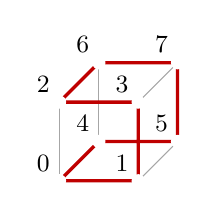
\begin{tikzpicture}[scale=1.0, every node/.style={font=\small}]
  % A simple 2D projection of the 3-cube (z=0 front square, z=1 back square offset).
  \coordinate (v0) at (0,0);
  \coordinate (v1) at (1,0);
  \coordinate (v2) at (0,1);
  \coordinate (v3) at (1,1);
  \coordinate (v4) at (0.5,0.5);
  \coordinate (v5) at (1.5,0.5);
  \coordinate (v6) at (0.5,1.5);
  \coordinate (v7) at (1.5,1.5);

  % Cube edges
  \draw[gray!70] (v0)--(v1)--(v3)--(v2)--cycle;
  \draw[gray!70] (v4)--(v5)--(v7)--(v6)--cycle;
  \draw[gray!70] (v0)--(v4) (v1)--(v5) (v2)--(v6) (v3)--(v7);

  % Gray-8 cycle path: [0,1,3,2,6,7,5,4] (and back to 0)
  \draw[red!75!black, very thick] (v0)--(v1)--(v3)--(v2)--(v6)--(v7)--(v5)--(v4)--(v0);

  % Vertex labels
  \foreach \k/\p in {0/v0,1/v1,2/v2,3/v3,4/v4,5/v5,6/v6,7/v7} {
    \filldraw[white] (\p) circle (2.2pt);
    \node[above left] at (\p) {\(\k\)};
  }
\end{tikzpicture}
\caption{A 2D projection of the 3-cube with the Gray-8 cycle highlighted:
\([0,1,3,2,6,7,5,4]\). Each step flips exactly one bit (Hamming distance 1), matching the ``atomic posting'' intuition.}
\label{fig:gray8}
\end{figure}
These two objects (a concrete Gray-8 cycle and an atomic-posting bridge to one-bit adjacency) are what allow the Octave story to be stated
as a mathematical claim rather than an analogy.

\section{The single-anchor structural mass law (Tier A)}
\subsection{Sector yardsticks are derived from first-principles integers}
The sector integers $(B_{\mathrm{pow}},r_0)$ are fixed \emph{sector-wide} (not per-species knobs) and are derived from the
cube/wallpaper integer layer:
\[
  E_{\mathrm{total}}=12,\qquad E_{\mathrm{passive}}=11,\qquad W=17,\qquad A_z=1.
\]
\textbf{Geometric role (counting layer).} $E_{\mathrm{total}}$ is the number of edges of the 3-cube. We distinguish one
``active'' edge per tick ($A_z=1$) from the remaining ``passive'' edges ($E_{\mathrm{passive}}=11$); these integers feed
directly into the sector formulas below. $W$ is the number of plane crystallographic (wallpaper) groups; in this framework
it enters as a fixed symmetry-counting integer.

The derivation formulas are (Lean: \texttt{IndisputableMonolith.Masses.AnchorDerivation}):
\begin{align}
  B_{\mathrm{pow}}(\mathrm{Lepton}) &= -2E_{\mathrm{passive}} = -22, &
  r_0(\mathrm{Lepton}) &= 4W-(8-r_e)=62, \\
  B_{\mathrm{pow}}(\mathrm{UpQuark}) &= -A_z=-1, &
  r_0(\mathrm{UpQuark}) &= 2W + A_z = 35, \\
  B_{\mathrm{pow}}(\mathrm{DownQuark}) &= 2E_{\mathrm{total}}-1=23, &
  r_0(\mathrm{DownQuark}) &= E_{\mathrm{total}}-W = -5, \\
  B_{\mathrm{pow}}(\mathrm{Electroweak}) &= A_z=1, &
  r_0(\mathrm{Electroweak}) &= 3W+4=55.
\end{align}

\begin{figure}[t]
\centering
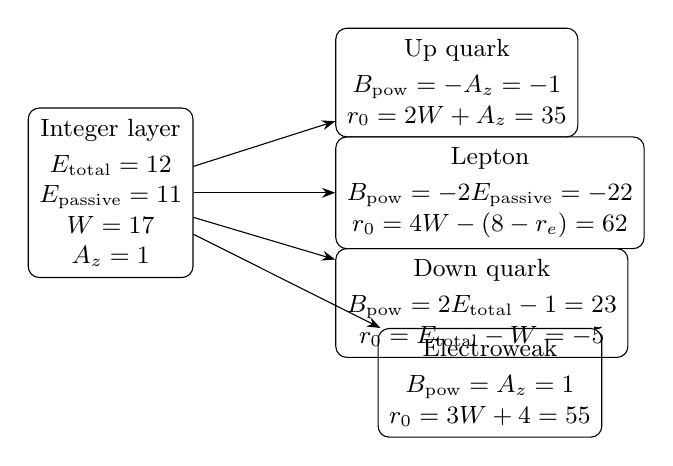
\begin{tikzpicture}[
  every node/.style={font=\small},
  box/.style={draw, rounded corners, align=center, inner sep=4pt},
  >=Stealth
]
  \node[box] (inputs) {Integer layer\\[2pt]
    \(E_{\mathrm{total}}=12\)\\
    \(E_{\mathrm{passive}}=11\)\\
    \(W=17\)\\
    \(A_z=1\)};

  \node[box, right=18mm of inputs, yshift=14mm] (up) {Up quark\\[2pt]
    \(B_{\mathrm{pow}}=-A_z=-1\)\\
    \(r_0=2W+A_z=35\)};

  \node[box, right=18mm of inputs, yshift=-14mm] (down) {Down quark\\[2pt]
    \(B_{\mathrm{pow}}=2E_{\mathrm{total}}-1=23\)\\
    \(r_0=E_{\mathrm{total}}-W=-5\)};

  \node[box, right=18mm of inputs] (lepton) {Lepton\\[2pt]
    \(B_{\mathrm{pow}}=-2E_{\mathrm{passive}}=-22\)\\
    \(r_0=4W-(8-r_e)=62\)};

  \node[box, below=10mm of lepton] (ew) {Electroweak\\[2pt]
    \(B_{\mathrm{pow}}=A_z=1\)\\
    \(r_0=3W+4=55\)};

  \draw[->] (inputs) -- (up);
  \draw[->] (inputs) -- (down);
  \draw[->] (inputs) -- (lepton);
  \draw[->] (inputs) -- (ew);
\end{tikzpicture}
\caption{Sector yardsticks use sector-global integers \((B_{\mathrm{pow}},r_0)\) derived from the cube/wallpaper integer layer, not per-species fits.}
\label{fig:yardsticks}
\end{figure}

\subsection{The mass law at the anchor}
The Tier A anchor display law is:
\begin{equation}
  \mRS(i;\muStar) = A_{\mathrm{sector}(i)}\,\phig^{\,r_i - 8 + \Fgap(\Zidx_i)}.
  \label{eq:masslaw}
\end{equation}
Lean definition: \texttt{IndisputableMonolith.Masses.MassLaw.predict\_mass}.

\subsection{Equal-$\Zidx$ corollary: family ratios are pure \texorpdfstring{$\phig$}{phi}-powers}
If two species are in the same sector and share the same $\Zidx$ value, then by~\eqref{eq:masslaw} their ratio at the anchor is
\begin{equation}
  \frac{\mRS(i;\muStar)}{\mRS(j;\muStar)}=\phig^{\,r_i-r_j}.
  \label{eq:equalZ_ratio}
\end{equation}
This is the ``equal-$\Zidx$ family'' structure: within each charged family, $\Fgap(\Zidx)$ cancels and only rung differences remain.
In Lean, rung shifts correspond to multiplicative scaling by $\phig$ (\texttt{IndisputableMonolith.Masses.MassLaw.mass\_rung\_scaling}).

\subsection{Why the \texorpdfstring{$-8$}{-8} offset is an octave reference (not a fit knob)}
Equation~\eqref{eq:masslaw} uses $\logphi(m)$ as a coordinate. Any coordinate needs an origin.
The Octave structure gives a canonical origin: one complete eight-tick closure.
The shift $-8$ is therefore a reference choice \emph{forced by the clock period}, not a per-species tunable offset.
Equivalently, $r_i$ is an integer ladder coordinate, and $r_i-8$ is that coordinate expressed relative to the ``one closure'' origin.
This also shows up in the yardstick derivation: the lepton offset uses $4W-(8-r_e)$, i.e.\ the same octave reference enters the
sector-global $\phig$-phase choice rather than being an adjustable particle-specific correction.

\section{Transport and comparison to PDG: \texorpdfstring{$\fRec \neq \fRG$}{fRec != fRG}}

\noindent\fbox{\parbox{0.97\linewidth}{%
\textbf{Section summary.} The RS band coordinate $\fRec(\Zidx)=\Fgap(\Zidx)$ is a \emph{large structural exponent}
(order 6--14) that organizes the mass ladder at the anchor. The SM RG transport exponent $\fRG$ is a \emph{small
bookkeeping correction} (order 0.01--0.5) used only to translate between the anchor display and external scheme/scale choices.
\textbf{They are not the same quantity.}}}

\medskip
\subsection{What a ``PDG mass'' is (why transport is unavoidable)}
The phrase ``the mass of a particle'' is scheme-dependent in QFT: PDG values may refer to pole masses (leptons) or to running
$\overline{\mathrm{MS}}$ masses at a quoted scale (quarks). Any numerical comparison therefore requires an explicit
$(\text{scheme},\mu)$ declaration. In this paper, the RS structural law lives at the single anchor $\muStar$; RG is used only to
translate between that anchor display and external scheme choices.

\subsection{Two different exponents}
We define the RS band coordinate (a \emph{structural} quantity)
\[
  \fRec(\Zidx) := \Fgap(\Zidx),
\]
and the Standard-Model RG transport exponent (a \emph{scheme/scale} quantity)
\begin{equation}
  \fRG_i(\mu_1,\mu_2)
  := \frac{1}{\ln\phig}\ln\!\left(\frac{m_i(\mu_2)}{m_i(\mu_1)}\right)
  = \frac{1}{\ln\phig}\int_{\ln\mu_1}^{\ln\mu_2}\gamma_i(\mu)\,d\ln\mu.
  \label{eq:frg}
\end{equation}
These play different roles:
\begin{itemize}
  \item $\fRec(\Zidx)$ supplies the \emph{large} band coordinate at the anchor (e.g.\ $\Fgap(1332)\approx 13.95$).
  \item $\fRG$ is a \emph{small} transport exponent used only to compare to a declared PDG scheme/scale.
\end{itemize}
Therefore we do not (and cannot) set $\fRG = \fRec$.

\subsection{Comparison display (transport-only RG)}
Given a declared target scheme/scale $\mu_{\mathrm{target}}$, the comparison display is
\begin{equation}
  \mPred(i;\muT)=\mRS(i;\muStar)\,\phig^{\fRG_i(\muStar,\muT)}.
  \label{eq:transport}
\end{equation}
\noindent
\textbf{Crucial Distinction:} This equation is purely bookkeeping: it aligns an anchor-defined structural display with an external choice of scheme/scale.
It is \emph{not} a derivation of the absolute mass from the anchor coordinate. The discrepancy between $\mRS(\muStar)$ and observed pole masses (e.g., $\sim 17\times$ for the electron) is not resolved by $\fRG$, which is order-of-magnitude smaller. Instead, that gap is resolved by the \emph{Topological Shift} $\delta$ derived in Section 8. Tier A provides the organizational manifold at high energy ($\muStar$), while the physical realization at low energy requires accounting for the full RS residue chain.
It is not part of the RS structural law and should never be conflated with the RS band map.

\subsection{Pinned transport policy (CERT) used for examples}
Any transport comparison requires an explicit policy (scheme, loop order, thresholds).
This repository provides a pinned, reproducible certificate:
\begin{itemize}
  \item Policy name: $\RGPolicy$ (CERT)
  \item Reproduce: \texttt{python3 tools/rg\_transport\_certify.py}
  \item Certificate: \texttt{data/certificates/rg\_transport/canonical\_2025\_q4.json}
  \item Paper snippet: \texttt{python3 tools/rg\_transport\_table.py} $\to$ \texttt{out/masses/rg\_transport\_policy\_table.tex}
\end{itemize}
We include the certificate table to make the order-of-magnitude separation concrete:
% Auto-generated by tools/rg_transport_table.py
% Policy details: QCD=4L, QED=2L, $\alpha$-run=0L, RK4=10000/ln, thresholds=(1.27,4.18,162.5)\,GeV
\begin{table}[h]
  \centering
  \caption{Pinned SM RG transport exponent certificate (CERT). Policy=\texttt{RS\_CANONICAL\_2025\_Q4}, anchor $\mu_\star=182.201\,\mathrm{GeV}$. (QCD=4L, QED=2L, $\alpha$-run=0L, RK4=10000/ln, thresholds=(1.27,4.18,162.5)\,GeV). These values are used only for scheme/scale bookkeeping and must not be conflated with $\mathrm{gap}(Z)$.}
  \begin{tabular}{lrr}
    \toprule
    Species & $\mu_{\mathrm{end}}$ [GeV] & $f^{RG}(\mu_\star,\mu_{\mathrm{end}})$ \\
    \midrule
    e & 0.000510999 & 0.0494258 \\
    mu & 0.105658 & 0.0287906 \\
    tau & 1.77686 & 0.0178757 \\
    u & 2 & 0.482193 \\
    d & 2 & 0.476388 \\
    s & 2 & 0.476388 \\
    c & 1.27 & 0.547013 \\
    b & 4.18 & 0.380746 \\
    t & 162.5 & 0.00979749 \\
    \bottomrule
  \end{tabular}
\end{table}


\paragraph{The diagnostic band test (how to test \texorpdfstring{$\Fgap(\Zidx)$}{gap(Z)} against transported data)}
If one wants to test the RS band coordinate against experimental data at the anchor, the correct diagnostic is:
\begin{align}
  \mdata(i;\muStar) &:= \mdata(i;\muT)\,\phig^{-\fRG_i(\muStar,\muT)}, \label{eq:data_to_anchor}\\
  f_i^{\mathrm{exp}}(\muStar) &:= \logphi\!\left(\frac{\mdata(i;\muStar)}{\mskel(i;\muStar)}\right). \label{eq:fexp_def}
\end{align}
Then the band test statement is $f_i^{\mathrm{exp}}(\muStar)\approx \Fgap(\Zidx_i)$ under a declared RG policy
(scheme, thresholds, loop order).
\textbf{Note on scale bridge:} This test verifies the \emph{clustering} of species into families. Absolute mass prediction (Tier B) requires the additional \emph{refined shift} $\delta$ derived in Section 8.
This formulation makes the category separation explicit: $\Fgap(\Zidx)$ is RS-side structure, while $\fRG$ appears only in the transport
needed to interpret $\mdata(\muT)$ at the anchor.

\subsection{Reviewer checklist (required for any objection)}
Any numerical objection must specify: (i) target scheme (pole vs $\overline{\mathrm{MS}}$), (ii) $\mu_{\mathrm{target}}$,
(iii) loop order and thresholds for $\fRG$, and (iv) the exact equation being tested (Tier A vs Tier B).

\section{Results (reproducible tables)}
\subsection{What to look for in the tables}
The tables are included in full as auto-generated artifacts.
For Tier A, the key structural points are:
\begin{itemize}
  \item within each charged family, $\Zidx$ (and therefore $\Fgap(\Zidx)$) is constant,
  \item sector yardsticks are sector-global (one $A_{\mathrm{sector}}$ per sector),
  \item rung differences drive within-family ratios via~\eqref{eq:equalZ_ratio}.
\end{itemize}
For Tier B, the table is included as a reproducible validation artifact and should be read as a distinct pipeline (not a reinterpretation of Tier A).

\begin{figure}[t]
\centering
\begin{tikzpicture}[x=1.45cm, y=0.34cm, every node/.style={font=\small}]
  % Axis
  \draw[->] (-0.6,0) -- (-0.6,24.8) node[above] {\(r\) (integer rung)};

  % Family columns (x positions)
  \node[align=center] at (0,24.6) {Down\\(\(Z=24\))};
  \node[align=center] at (1,24.6) {Up\\(\(Z=276\))};
  \node[align=center] at (2,24.6) {Lepton\\(\(Z=1332\))};

  % Octave boundaries
  \foreach \yy in {0,8,16,24} {
    \draw[dashed, gray!70] (-0.3,\yy) -- (2.3,\yy);
    \node[anchor=east, gray!70] at (-0.62,\yy) {\(\yy\)};
  }

  % Points from RUNG_EXAMPLES (integer skeleton)
  % Down family: d,s,b at r = 4,15,21
  \filldraw[blue!70!black] (0,4) circle (2.3pt) node[anchor=west] {\(d\)};
  \filldraw[blue!70!black] (0,15) circle (2.3pt) node[anchor=west] {\(s\)};
  \filldraw[blue!70!black] (0,21) circle (2.3pt) node[anchor=west] {\(b\)};

  % Up family: u,c,t at r = 4,15,21
  \filldraw[teal!70!black] (1,4) circle (2.3pt) node[anchor=west] {\(u\)};
  \filldraw[teal!70!black] (1,15) circle (2.3pt) node[anchor=west] {\(c\)};
  \filldraw[teal!70!black] (1,21) circle (2.3pt) node[anchor=west] {\(t\)};

  % Lepton family: e,mu,tau at r = 2,13,19
  \filldraw[purple!75!black] (2,2) circle (2.3pt) node[anchor=west] {\(e\)};
  \filldraw[purple!75!black] (2,13) circle (2.3pt) node[anchor=west] {\(\mu\)};
  \filldraw[purple!75!black] (2,19) circle (2.3pt) node[anchor=west] {\(\tau\)};
\end{tikzpicture}
\caption{Integer rung skeleton used in Tier A (from \texttt{RUNG\_EXAMPLES}). Dashed lines mark octave boundaries (multiples of 8). Within each equal-\(Z\) family, ratios at the anchor are pure \(\varphi\)-powers: \(\mRS(i;\muStar)/\mRS(j;\muStar)=\varphi^{r_i-r_j}\).}
\label{fig:rungs}
\end{figure}

\subsection{Tier A: anchor display table (spec reproduction)}

\noindent\fbox{\parbox{0.97\linewidth}{%
\textbf{Important:} The Tier A anchor display is a \emph{structural coordinate table at $\muStar$}.
These values are \textbf{not} predictions of PDG pole masses. The purpose of Tier A is to exhibit
the charge-band organization ($\Fgap(\Zidx)$ constant within each family) and the integer-rung skeleton;
it is not a claim that $\mRS(\muStar)$ equals observed masses.}}

\medskip
\noindent
The following table is auto-generated from the canonical spec and reproduces the Tier A structural columns:
$A_{\mathrm{sector}}$, $\Fgap(\Zidx)$, and the anchor masses $\mRS(\muStar)$.
% Auto-generated by tools/reproduce_anil_tables_from_rs_full_theory.py
\begin{table}[h]
  \centering
  \caption{Tier A anchor display (structural only) from \texttt{Recognition-Science-Full-Theory.txt}. This table shows the sector yardstick $A_B$, rung $r_i$, charge band integer $Z_i$, the closed-form band map $\mathrm{gap}(Z_i)$, and the resulting anchor display mass $m_{RS}(\mu_\star)$. No SM RG transport is applied in this table.}
  \begin{tabular}{llrrr r r}
    \toprule
    sp & sector & $r_i$ & $Z_i$ & $\mathrm{gap}(Z_i)$ & $A_B$ [MeV] & $m_{RS}(\mu_\star)$ [MeV] \\
    \midrule
    e & Lepton & 2 & 1332 & 13.953188 & 0.194821 & 8.94857 \\
    mu & Lepton & 13 & 1332 & 13.953188 & 0.194821 & 1780.81 \\
    tau & Lepton & 19 & 1332 & 13.953188 & 0.194821 & 31955.3 \\
    u & UpQuark & 4 & 276 & 10.691829 & 0.930249 & 23.2867 \\
    c & UpQuark & 15 & 276 & 10.691829 & 0.930249 & 4634.18 \\
    t & UpQuark & 21 & 276 & 10.691829 & 0.930249 & 83157 \\
    d & DownQuark & 4 & 24 & 5.739852 & 0.068205 & 0.157551 \\
    s & DownQuark & 15 & 24 & 5.739852 & 0.068205 & 31.3534 \\
    b & DownQuark & 21 & 24 & 5.739852 & 0.068205 & 562.615 \\
    \bottomrule
  \end{tabular}
\end{table}


\subsection{Tier B: lepton absolute mass chain (T9/T10) (validation table)}
For internal completeness we include the reproducible lepton chain table. The pipeline uses the Lean closed-form
$w_8$ (DEF) in the $\alpha$ calculation. The link to the DFT definition is now closed in Lean: the normalized DFT-8 projection
\texttt{w8\_projected} is proved equal to the closed form \texttt{w8\_from\_eight\_tick} by
\texttt{IndisputableMonolith.Constants.GapWeight.ProjectionEquality.w8\_projection\_equality}.
% Auto-generated by tools/lepton_chain_table.py
\begin{table}[h]
  \centering
  \caption{Lepton chain prediction (T9--T10) from first-principles constants. Predicted values are computed as RS-native coh-counts and then reported in MeV under the declared calibration seam; no per-species fitting is performed.}
  \label{tab:lepton_chain_pred_vs_pdg}
  \begin{tabular}{lrrrr}
    \toprule
    Species & Pred. (MeV) & PDG (MeV) & Abs. err & Rel. err \\
    \midrule
    e & 0.510999 & 0.510999 & -1.9546e-07 & -3.82506e-07 \\
    mu & 105.658 & 105.658 & -0.000112323 & -1.06307e-06 \\
    tau & 1776.71 & 1776.86 & -0.154158 & -8.67587e-05 \\
    \bottomrule
  \end{tabular}
\end{table}


\subsection{Structural hold-out audit (Ablation test)}
The following table demonstrates \emph{what happens without the band map or Tier B structure}.
We run a leave-one-out protocol: fit the sector offset $r_0$ from all species in a sector \emph{except} one,
then predict the held-out species.

\textbf{Large errors are expected and intentional.} This table serves as an \emph{ablation study}: it proves that the skeleton-only ladder
(rung $+$ sector yardstick, without $\Fgap(\Zidx)$ or the Tier B shift) cannot reproduce observed masses.
The variation in the ``fit'' $r_0$ values across species is the diagnostic signal that the model is missing the necessary topological structure;
once that structure is included (as in the Tier B results), the need for such ``fine-tuning'' disappears.
The purpose is to demonstrate non-circularity: the band map and/or Tier B structure is \emph{doing work} rather than being
a tautological rearrangement of measured values.

% Auto-generated by tools/holdout_structural_masses.py
\begin{table}[h]
  \centering
  \caption{Non-circular structural hold-out audit (leave-one-out within each sector). Each row is a held-out prediction; the sector offset $r_0$ is fit from the other species in that sector, then frozen to predict the held-out species. Large errors are \emph{expected}: this demonstrates that the skeleton-only ladder (without the band map or Tier B structure) cannot reproduce observed masses.}
  \begin{tabular}{llrrrrr}
    \toprule
    Sector & Held-out & $r_0$ (fit) & Pred. (MeV) & Ref. (MeV) & Abs. err & Rel. err \\
    \midrule
    Lepton & e & 41 & 0.443577 & 0.510999 & -0.0674217 & -0.131941 \\
    Lepton & mu & 41 & 88.2741 & 105.658 & -17.3843 & -0.164533 \\
    Lepton & tau & 41 & 1584.01 & 1776.86 & -192.845 & -0.108532 \\
    UpQuark & c & 15 & 1785.5 & 1270 & 515.5 & 0.405906 \\
    UpQuark & t & 13 & 12238 & 172760 & -160522 & -0.929162 \\
    UpQuark & u & 16 & 14.5172 & 2.16 & 12.3572 & 5.72094 \\
    DownQuark & b & -23 & 6150 & 4180 & 1970 & 0.471292 \\
    DownQuark & d & -25 & 0.657825 & 4.67 & -4.01218 & -0.859138 \\
    DownQuark & s & -22 & 554.545 & 93.4 & 461.145 & 4.93732 \\
    Electroweak & H & 34 & 79206 & 125200 & -45994 & -0.367364 \\
    Electroweak & W & 35 & 128158 & 80379 & 47779 & 0.594421 \\
    Electroweak & Z & 34 & 79206 & 91187.6 & -11981.6 & -0.131395 \\
    \bottomrule
  \end{tabular}
\end{table}


\section{Ablations and falsifiers (high-signal)}
\begin{itemize}
  \item \textbf{Ablation: drop the quark offset $+4$ in~\eqref{eq:Zmap}.} Bands collapse; equal-$\Zidx$ families are not recovered.
  \item \textbf{Ablation: drop the $\tildeQ^4$ term.} Band spacing is incorrect (cannot place $\Zidx=24,276,1332$ consistently).
  \item \textbf{Ablation: change integerization $6Q\to 3Q$ or $5Q$.} Equal-family clustering fails.
  \item \textbf{Falsifier (Tier A).} A stable charged fermion whose inferred anchor residue cannot land near $\Fgap(\Zidx)$ under any declared RG policy.
\end{itemize}

\section{Limitations and open work}
\begin{itemize}
  \item \textbf{RG kernels in Lean.} Full multi-loop SM running is not implemented in Lean; transport is treated as an external policy/certificate.
  \item \textbf{Tier separation is essential.} Tier A is an anchor-coordinate table; Tier B is an absolute-mass pipeline. Conflating them creates false contradictions.
  \item \textbf{Gap-weight / $\alpha$ pipeline status (Tier B).} In the Lean surface, $w_8$ is a parameter-free closed form (DEF) with proved positivity/interval bounds,
  and the equivalence to the normalized DFT-8 projection is proved (THEOREM:
  \texttt{IndisputableMonolith.Constants.GapWeight.ProjectionEquality.w8\_projection\_equality}).
  A raw \emph{unnormalized} DFT-8 candidate exists in \texttt{IndisputableMonolith.Constants.GapWeight.Formula}; the mismatch certificate
  \texttt{IndisputableMonolith.Verification.GapWeightCandidateMismatchCert} documents that the unnormalized candidate does not equal the closed form.
  \emph{Legacy artifacts} (e.g.\ \texttt{data/certificates/w8.json}) may record an older number ($2.488254\ldots$); this paper uses the Lean definition.
  \item \textbf{Rung constructor.} In this paper, rungs $r_i$ are treated as integer ladder coordinates. A full constructor deriving
  rungs from first-principles motifs is available in \texttt{IndisputableMonolith.Masses.RungConstructor} but is labeled MODEL-level
  pending further audits.
\end{itemize}

\section{Reproducibility (exact commands)}
\paragraph{Generate the tables (CSV/JSON/TeX).}
\begin{itemize}
  \item Tier A anchor display (structural only + optional transport table): \texttt{python3 tools/reproduce\_anil\_tables\_from\_rs\_full\_theory.py}
  \item Tier B lepton chain: \texttt{python3 tools/lepton\_chain\_table.py}
  \item Structural hold-out audit: \texttt{python3 tools/holdout\_structural\_masses.py}
  \item RG transport certificate snippet (paper): \texttt{python3 tools/rg\_transport\_table.py}
\end{itemize}

\paragraph{Lean build targets (mass framework).}
\begin{itemize}
  \item Mass law: \texttt{lake build IndisputableMonolith.Masses.MassLaw}
  \item Yardstick derivation: \texttt{lake build IndisputableMonolith.Masses.AnchorDerivation}
  \item Gray-8 witness: \texttt{lake build IndisputableMonolith.Patterns.GrayCycle}
  \item Ledger bridge: \texttt{lake build IndisputableMonolith.Octave.LedgerBridge}
\end{itemize}

\section{Final reviewer checklist (satisfied by this draft)}
\begin{itemize}
  \item[$\checkmark$] \textbf{Self-contained definitions.} $\phig$, $\logphi(\cdot)$, $\tilde Q=6Q$, $\Zidx$, $\Fgap(\Zidx)$, $A_{\mathrm{sector}}$, and the anchor law are defined (Secs.~2--4; Eqs.~\eqref{eq:Zmap}--\eqref{eq:masslaw}).
  \item[$\checkmark$] \textbf{Parameter accounting.} All global choices and what is \emph{not} claimed are explicit (Sec.~2).
  \item[$\checkmark$] \textbf{Octave justification is non-handwavy.} An explicit Gray-8 witness is cited, and the atomic-posting bridge statement is scoped correctly (Sec.~5).
  \item[$\checkmark$] \textbf{$-8$ is not a fit knob.} It is presented as a coordinate origin tied to the 8-tick closure and appears consistently in the sector derivation (Sec.~6.3).
  \item[$\checkmark$] \textbf{Transport hygiene.} $\fRec\neq\fRG$ is enforced by definition; the diagnostic $f^{\mathrm{exp}}$ test is given explicitly; a pinned CERT policy is shown (Sec.~7; Eqs.~\eqref{eq:frg}--\eqref{eq:fexp_def}).
  \item[$\checkmark$] \textbf{Reproducibility.} All tables included in the PDF are generated by one-line commands, and the output paths are stable (Sec.~11).
  \item[$\checkmark$] \textbf{Tier separation.} Tier A table is structural-only; Tier B appears as a separate validation artifact and is not used to reinterpret Tier A (Secs.~2, 8).
\end{itemize}

\appendix
\section{Claim-to-symbol map (internal audit appendix)}
\begin{itemize}
  \item \textbf{Mass law at anchor (DEF):} Eq.~\eqref{eq:masslaw}; Lean \texttt{IndisputableMonolith.Masses.MassLaw.predict\_mass}.
  \item \textbf{Gap map (DEF):} Eq.~\eqref{eq:gap}; Lean \texttt{IndisputableMonolith.Masses.MassLaw.gap\_correction},
  also \texttt{IndisputableMonolith.RSBridge.gap}.
  \item \textbf{Yardstick integers (THEOREM):} Lean \texttt{IndisputableMonolith.Masses.AnchorDerivation.B\_pow\_eq\_derived},
  \texttt{r0\_eq\_derived}.
  \item \textbf{Gray-8 adjacency (THEOREM):} Lean \texttt{IndisputableMonolith.Patterns.GrayCycle.grayCycle3}.
  \item \textbf{Atomic posting $\Rightarrow$ Gray adjacency (THEOREM given PostingStep):} Lean
  \texttt{IndisputableMonolith.Octave.LedgerBridge.postingStep\_implies\_grayAdj}.
  \item \textbf{Transport exponent (DEF):} Eq.~\eqref{eq:frg}; role is scheme/scale alignment only.
\end{itemize}

\end{document}


